\documentclass[10pt,a4paper]{article}
\usepackage[utf8]{inputenc}
\usepackage[margin=1.5cm]{geometry}
\usepackage{enumitem}
\usepackage{titlesec}
\usepackage{hyperref}
\usepackage{graphicx}
\usepackage{fontawesome5}
\usepackage{array}
\usepackage{longtable}
\usepackage[none]{hyphenat}
\usepackage{makecell}  % fix \makecell error

% CV section formatting

\newcommand{\cvsection}[3][1.2]{%
  \renewcommand{\arraystretch}{1} % Reset to default for header
  \faCaretRight \; \textbf{#2}

  \renewcommand{\arraystretch}{#1}% Apply custom row spacing
  \begin{longtable}{
    >{\raggedleft\arraybackslash}p{0.20\textwidth}
    @{\hspace{1cm}}
    >{\raggedright\arraybackslash}p{0.68\textwidth}
  }
    \endfirsthead
    \endhead
    \endfoot
    \endlastfoot
    #3
  \end{longtable}

  \renewcommand{\arraystretch}{1}% Reset to default
  \vspace{1em}%
}

% Remove page numbers
\pagestyle{empty}

% Customize section headings
\titleformat{\section}{\large\bfseries\uppercase}{}{0em}{}[\titlerule]
\titlespacing{\section}{0pt}{12pt}{6pt}

\begin{document}

% Header
\begin{minipage}[c]{0.65\textwidth}
    Email: alessandro.pedone02@gmail.com \\
    Phone: +39 345 705 3904 \\
    LinkedIn: \href{https://linkedin.com/in/alessandro-pedone-58288a368/}{\faLink} \\
    GitHub: alessandropedone \href{https://github.com/alessandropedone}{\faLink} \\
    Location: 20143 Milan, Italy \\

\end{minipage}
\hfill
\begin{minipage}[c]{0.3\textwidth}
    \raggedleft
    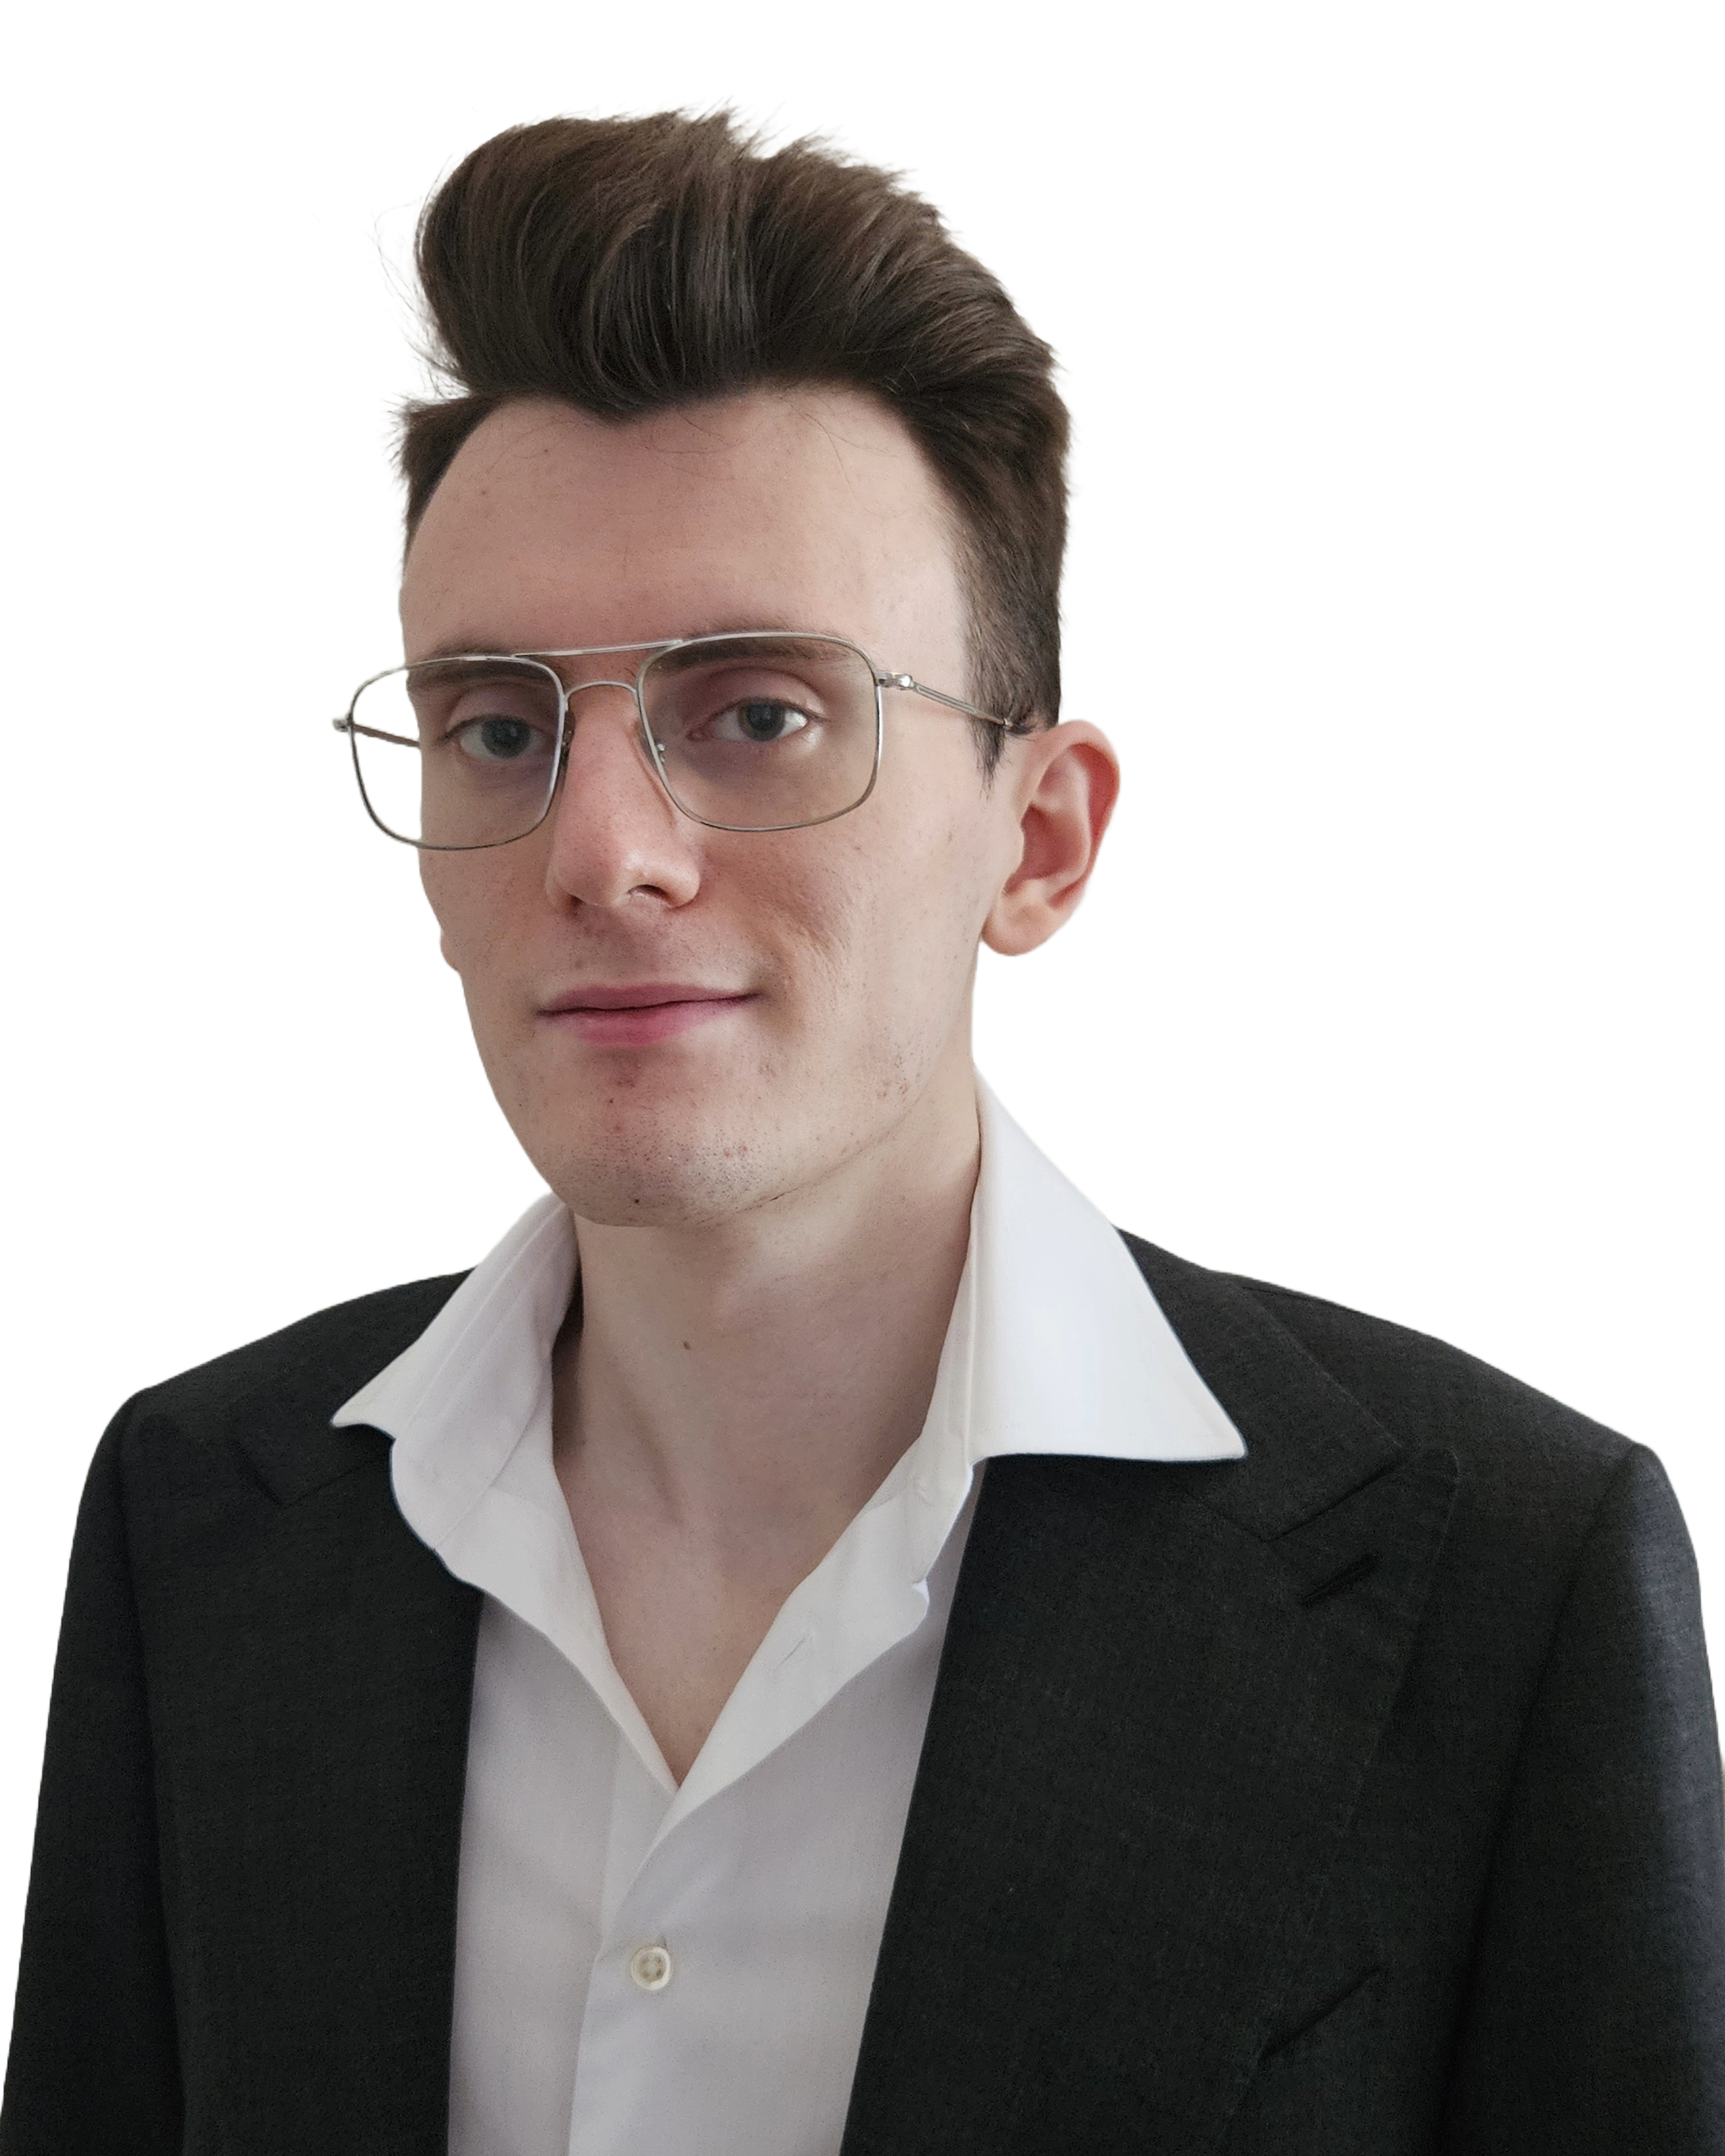
\includegraphics[width=3cm,height=3cm,keepaspectratio]{photo.jpg}
\end{minipage}

\vspace{12pt}
\begin{center}
    {\LARGE\bfseries Alessandro Pedone} \\
    \vspace{1em}
    {\LARGE\bfseries Curriculum Vitae} \\
\end{center}

\vspace{12pt}

\small{

    \cvsection{PERSONAL DATA}{
        Date of Birth & 01/10/2002 \\
        Nationality & Italian \\
        Place of Birth & Milan, Italy \\
    }

    \cvsection{CURRENT POSITION}{
        Politecnico di Milano & Pursuing Master's Degree in Mathematical Engineering,
        with a focus on Computational Science and Computational Learning\\
    }

    \cvsection{AREAS OF INTEREST}{
        &  Scientific Machine Learning\\
        & Numerical Analysis \\
        & Partial Differential Equations (PDEs) \\
        & Mathematical Analysis \\
    }

    \cvsection{EDUCATION}{
        2024 - Current &   \textbf{Master's Degree in Mathematical Engineering, Politecnico di Milano} \\
        & \\
        2021 - 2024 & \textbf{Bachelor's Degree in Mathematical Engineering, Politecnico di Milano} \\
        & Final grade: 110/110 cum laude \\
        & Thesis: The Cauchy-Kowalevski theorem and some of its consequences \\
        & Keywords: PDEs, characteristics method, analyticity/holomorphy, power series, method of majorants, Cauchy-Kowalevski, Holmgren and Cartan-Kähler theorems \\
        & Supervisor: Prof. Maurizio Grasselli
    }

    \cvsection{EXPERIENCE}{

        27/10/2025 - 31/10/2025 &  \textbf{Scientific Machine Learning and Numerical Methods - Autumn School} \\
        & \textit{Admitted (as a Master's student) to a highly selective PhD program organized by CWI
            (Centrum Wiskunde \& Informatica), primarily comprising PhD candidates.} \\
        & Topics:
        \begin{itemize}[leftmargin=*,nosep,label={\tiny$\bullet$}]
            \item Differential equations and data-driven modeling
            \item Optimization for inverse problems
            \item Probabilistic numerical methods
            \item Physics-informed machine learning
            \item Stochastic processes and computational efficiency
        \end{itemize}\\
        23/06/2025 - 27/06/2025 & \textbf{Theorical Foundations of Machine Learning 2025} \\
        & \textit{Admitted (as a Master's student) to a highly selective PhD program organized
            by MaLGa (Machine Learning Genoa Center) at the University of Genoa,
            with an acceptance rate of approximately 10\%, primarily comprising PhD candidates.} \\
        & Topics:
        \begin{itemize}[leftmargin=*,nosep,label={\tiny$\bullet$}]
            \item Statistical learning theory framework
            \item Kernel methods and neural networks
            \item Empirical risk minimization and regularization
            \item Reproducing kernel Hilbert spaces (RKHS)
            \item Optimization techniques: convex analysis, gradient methods, stochastic
                  optimization, splitting methods, backpropagation
            \item Theoretical analysis: concentration inequalities, empirical process theory,
                  spectral calculus, operator theory
        \end{itemize}
    }

    \cvsection{HONOURS AND AWARDS}{
        25/01/2023 &   \textbf{Premio Migliori Matricole aa 21-22 Classe L 8 Fondo Giovani} \\
        & Best Freshmen Award, academic year 2021–2022, Class L-8, Fondo Giovani — granted upon completion of the first year of enrollment, based on academic performance, including GPA and the number of ECTS credits earned.
    }

    \cvsection{MEMBERSHIPS}{
        2025 - Current &   SIAM (Society for Industrial and Applied Mathematics) \\
        \\
        2021 – Current & AIM (Associazione Ingegneri Matematici)
    }

    \cvsection{VOLUNTEERING}{
        2020 - Current &   Blood donor \\
        2018 & ABCDigital: Liceo Scientifico Elio Vittorini promoted a project to organize a free course for senior citizens,
        consisting of 10 weekly lectures (2 hours each), aimed at improving their digital skills,
        device usage, and online awareness.
    }

    \cvsection{LANGUAGES}{
        Italian &  Native speaker \\
        English & C1 (IELTS 7.5) \\
    }

    \cvsection{SKILLS}{
        Programming Languages &    Python, C/C++, MATLAB, R, LaTeX \\
        Libraries & NumPy, SciPy, scikit-learn, TensorFlow, Keras, Pandas, Matplotlib, Seaborn, MIP, FEniCS, FEniCSx\\
        Operating Systems & Linux (Ubuntu), Windows \\
        Additional Software & Notion \\
        Other skills: Method of loci, Mnemonic major system, Mnemonic link system
    }

    \cvsection{PROJECTS}{
        04/2025 - Current &    \textbf{Coupling CGA-DL-ROM with traditional solver for multiphysics problem} \\
        & Reference: \href{https://arxiv.org/abs/2411.05486v1}{\faLink} \\
        & Objective: perform simulation of a simplified MEMS dynamics.\\
        & Dataset: 1000 meshes with the corresponding solutions of the problem.\\
        & Methodology:
        \begin{enumerate}[leftmargin=*,nosep]
            \item Built the meshes making 3 geometric parameters of the domain vary.
            \item Use traditional FEM solver to obtain the solution (of the electrical part of
                  the problem) for each case.
            \item Train a neural network (GCA-DL-ROM) as a surrogate model for this problem.
            \item Couple this efficient ROM with a traditional solver (for the mechanical part of
                  the problem) to obtain the motion inside the MEMS.
        \end{enumerate}\\

        04/2025 - Current & \textbf{Coupling MPE and Stokes' equations for cerebrospinal fluid flow and tissue motion} \\
        & Reference: \href{https://fluidsbarrierscns.biomedcentral.com/articles/10.1186/s12987-022-00376-2}{\faLink} \\
        & Objective: study cerebrospinal fluid (CSF) flow, inside brain ventricles and subarachnoid space, with a focus on modeling the latter and exploiting already existing results. \\
        & Dataset: not publicly available. \\
        & Methodology:
        \begin{enumerate}[leftmargin=*,nosep]
            \item \textit{Implementation challenges:} segmenting the geometry (obtained from MRI) and
                  creating the mesh of the subarachnoid space.
            \item \textit{Mathematical model:} coupling of MPE for brain tissue poromechanics Stokes'
                  equations for cerebrospinal fluid flow.
            \item \textit{Numerical tools:} high order discontinuous Galerkin method on polytopal meshes
                  for spatial discretization.
        \end{enumerate}\\

        03/2025 - 05/2025 & \textbf{C++ Scientific Computing Projects} \\
        & \begin{enumerate}[leftmargin=*,nosep]
            \item Some optimization methods for real-valued functions (Gradient Descent, Heavy
                  Ball, Nesterov, ADAM...)
            \item Parallel implementations of two kind of solvers for the Poisson equation in the
                  unit square (Schwarz method)
            \item Implementation of a matrix class, particularly suited for sparse matrices
                  (CSR/CSC formats and modified formats)
        \end{enumerate}\\

        12/2024 & \textbf{Mars Terrain segmentation} \\
        & Objective: segment Mars terrain images into five classes: Background, Soil, Bedrock, Sand, and Big Rock.\\
        & Dataset: 2,615 grayscale images (64x128 resolution), filtered to 2,505 images.\\
        & Methodology:
        \begin{enumerate}[leftmargin=*,nosep]
            \item Built an initial encoder-decoder architecture as benchmark.
            \item Added layer for Edge Detection, Thresholding and others methods of computer
                  vision.
            \item Implemented a dual UNet architecture (Global and Local perspectives).
            \item Designed custom loss functions and loss schedules.
            \item Applied data augmentation and fine-tuned optimization hyperparameters.
        \end{enumerate}\\

        11/2024 & \textbf{Blood Cell Classification} \\
        & Objective: perform an 8-class classification task on blood cells images.\\
        & Dataset: 13,759 RGB images (96x96 resolution), filtered to 11,959 images after preprocessing.\\
        & Methodology:
        \begin{enumerate}[leftmargin=*,nosep]
            \item Built an initial CNN architecture with regularization and augmentation as benchmark.
            \item Implemented Transfer Learning (TL) and Fine Tuning (FT).
            \item Deployed an ensemble of the best-performing models.
        \end{enumerate}\\

        04/2024 – 06/2024 & \textbf{Statistical Inference for Math Performance} \\
        & Objective: build a linear regression model for math perfomance of italian high school students.\\
        & Dataset: OECD PISA 2022 survey.\\
        & Methodology:
        \begin{enumerate}[leftmargin=*,nosep]
            \item Non-parametric ANOVA (Kruskal-Wallis and Dunn's test).
            \item Removal of influential points (outliers and leverages).
            \item Cross-validation.
            \item Prediction and confidence intervals.
        \end{enumerate}\\
    }
}
\end{document}